\documentclass[xcolor=pdftex,table,11pt]{beamer}
\usetheme{Warsaw}
\usepackage[utf8]{inputenc}
\usepackage[english]{babel}
\usepackage{amsmath}
\usepackage{amsfonts}
\usepackage{amssymb}
\usepackage{multirow}
\usepackage{siunitx}
\usepackage{listings}
\usepackage{tabulary}


\usepackage[highlightcolor=yellow]{../styles/code}
\author{Informática I - Instituto Unviersitario Areonáutico}
\title{Introducción a la programación en C}

\usepackage{booktabs}
\usepackage{longtable}
\newcommand*{\thead}[1]{\multicolumn{1}{c}{\bfseries #1}}

\usepackage{tikz}
\def\checkmark{\tikz\fill[scale=0.3](0,.35) -- (.25,0) -- (1,.7) -- (.25,.15) -- cycle;} 

%\setbeamercovered{transparent} 
%\setbeamertemplate{navigation symbols}{} 
%\logo{} 
%\institute{} 
%\date{} 
%\subject{} 
\begin{document}

\begin{frame}{Situación problemática}

\begin{block}{}
Se necesita tomar la lectura de temperatura y humedad de una estación meteorológica. La misma, toma una muestra cada una hora. \\
Al final del día, se debe imprimir una tabla con los valores tomados e informar los valores máximos y mínimos de cada una de las variables.
\end{block}
\end{frame}

\begin{frame}{Solución propuesta}


\codesetstylefrombeamer
\cppfile{../../c/arrays/1-problem_without_arrays.c}

\end{frame}

\begin{frame}{Arreglos unidimensionales}
\begin{block}{Introducción}
Un arreglo es una colección de variables del \textbf{mismo tipo} que están referenciadas por un nombre en común. 
\end{block}

\begin{figure}
 \centering
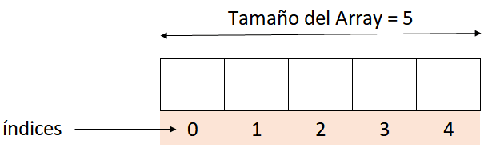
\includegraphics[scale=0.5]{../img/exported/arrays.png}
\caption{Representación de un arreglo unidimensional de cinco elementos.}
\end{figure}
\end{frame}


\begin{frame}{Arreglos unidimensionales}
\begin{block}{¿Cómo lo vemos desde C?}
Se puede pensar a un arreglo como un conjunto de posiciones de memoria contiguas, agrupadas bajo el mismo nombre. La dirección mas baja corresponde al primer elemento y las mas alta al último.
\end{block}

\begin{figure}
 \centering
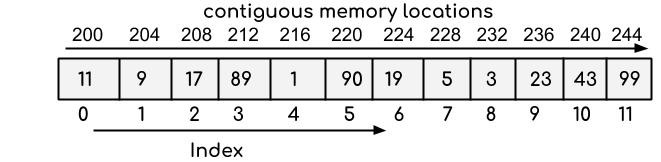
\includegraphics[scale=0.5]{../img/exported/array_with_memory.jpg}
\caption{Representación de un arreglo unidimensional de cinco elementos.}
\end{figure}

\textbf{Notar que el primer elemento de un arreglo es el 0.}

\end{frame}

\begin{frame}{Arreglos unidimensionales}
\begin{block}{¿Cuánto ocupa cada dato en memoria?}
Los arreglos en C tienen tamaño estático, es decir que al ejecutarse el programa mantendrá una cantidad fija de memoria reservada.

\end{block}
\vspace{0.5cm}

\begin{tabular}{|c|c|}
\hline 
\textbf{Tipo de datos} & \textbf{Tamaño en bytes} \\ 
\hline 
char - unsigned char & 1\\ 
\hline 
short int, unsigned short int & 2 \\ 
\hline 
int, unsigned int, long int, unsigned long int & 4 \\ 
\hline 
float & 4 \\ 
\hline 
double & 8 \\ 
\hline
long double & 12\\ 
\hline 
\end{tabular} 
\vspace{0.3cm}
\\
El tamaño en bytes puede cambiar de una plataforma a otra.


\href{https://www.profesionalreview.com/2018/12/12/unidades-de-medida/}{\beamergotobutton{Más información sobre bits y bytes}}

\end{frame}


\begin{frame}{Declaración de un arreglo unidimensional}
La forma general de declarar a un arreglos es:

\codesetstylefrombeamer
\cppfile{../../c/arrays/1-array_declarations.c}

Los nombres de los arreglos pueden contener letras, números  y guiones bajos.\\

\vspace{0.5cm}
Para declarar e inicializar un arreglo:
\cppfile{../../c/arrays/1-array_init.c}
\end{frame}



\begin{frame}{¿Cómo accedemos a los elementos de un arreglo?}
Se puede hacer referencia a cualquiera de los elementos de un arreglo  utilizando el nombre del mismo y el operador []. \\
En su interior, debe ir un número entero o una expresión entera. \\
Por ejemplo:

\codesetstylefrombeamer
\cppfile{../../c/arrays/1-array_access.c}

Las lineas 8,9 y 10 son equivalentes.\\

¿Si tenemos que cargar, recorrer y procesar un arreglo de 1000 elementos?
\end{frame}



\begin{frame}[allowframebreaks]{Vamos a C}
Carga de datos a un arreglo:
\codesetstylefrombeamer
\cppfile{../../c/arrays/1-array_load.c}

\newpage
Impresión del arreglo anterior:
\codesetstylefrombeamer
\cppfile{../../c/arrays/1-array_print.c}


\href{https://github.com/danis963/informaticaI_IUA/blob/main/c/src/8-array_load_print.c}{\beamergotobutton{Ver ejemplo en github}}

\textbf{Se debe tener en cuenta que C no tiene mecanismos de control de acceso a memoria, es decir que si un arreglo tiene 10 elementos y se intenta escribir la posición 19 podrían sobre-escribirse valores de otras variables. \\
Es responsabilidad del desarrollador hacer este control.}

\end{frame}


\begin{frame}{La directiva Define}
Una directiva (o macro) es resuelta por el preprocesador antes del proceso de compilación y reemplaza cada una de las etiquetas definidas, por su valor definido en la etiqueta.\\
\vspace{0.5cm}
Ejemplo antes de la compilación:
\codesetstylefrombeamer
\cppfile{../../c/arrays/1-define.c}

Ejemplo luego de la compilación:
\codesetstylefrombeamer
\cppfile{../../c/arrays/1-define_ac.c}


\vspace{0.5cm}
Como se ve, utilizando esta directiva se pueden desarrollar algoritmos genéricos independientes de la cantidad de elementos del arreglo.



\end{frame}




\begin{frame}{Ejemplos de arreglos unidimensionales}
 \begin{enumerate}
   
        \item Diseñar y codificar un programa que cargue un arreglo de 1000 elementos con números aleatorios comprendidos entre 10 y 20.\\
   Luego el programa debe recorrer el arreglo y contar las veces que un número ingresado por teclado aparece en el arreglo.
\href{https://github.com/danis963/informaticaI_IUA/blob/main/c/src/8-0-arrays.c}{\beamergotobutton{Ver en github}}


     \item Diseñar y codificar un programa que solicite el ingreso por teclado de 10 números enteros y los almacene en un arreglo unidimensional. Luego, se deben convertir los números positivos en negativos y los negativos en positivos.\\
Finalmente, se debe imprimir el arreglo original y el arreglo convertido.
\href{https://github.com/danis963/informaticaI_IUA/blob/main/c/src/8-1arrays.c}{\beamergotobutton{Ver en github}}

        \item Diseñar y codificar un programa que permita el ingreso de las mediciones de temperatura y humedad de una estación meteorológica. La misma, toma una muestra cada 1h. \\
        Al final del día se debe imprimir la temperaturas y humedades máximas y mínimas.
\href{https://github.com/danis963/informaticaI_IUA/blob/main/c/src/8-2arrays.c}{\beamergotobutton{Ver en github}}

   \end{enumerate}
\end{frame}



\begin{frame}{Arreglos Bidimensionales}
\begin{block}{}
Los arreglos bidimensionales son útiles cuando se debe trabajar con información ordenadas en filas y columnas.\\
Por convención, el primer índice indica la fila del elemento y el segundo la columna.
\end{block}

\begin{figure}
 \centering
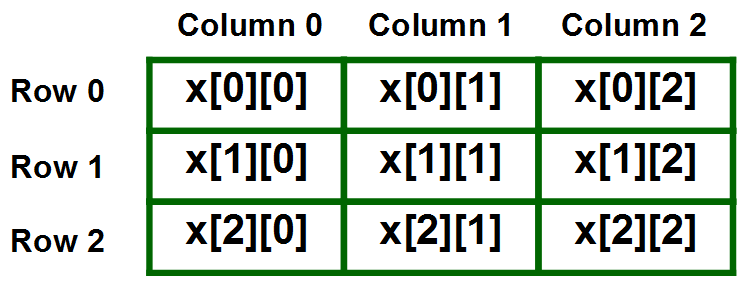
\includegraphics[scale=0.5]{../img/exported/matrix.png}
\caption{Representación de un arreglo bidimensional de 3x3.}
\end{figure}

\end{frame}


\begin{frame}{Declaración de un arreglo bidimensional}

\codesetstylefrombeamer
\cppfile{../../c/arrays/2-array_declarations.c}
\vspace{0.5cm}
\vspace{0.5cm}
Para declarar e inicializar un arreglo bidimensional, 
\codesetstylefrombeamer
\cppfile{../../c/arrays/2-array_init.c}


\end{frame}

\begin{frame}{Carga de un arreglo bidimensional}
\codesetstylefrombeamer
\cppfile{../../c/arrays/2-array_2d_init.c}
\end{frame}

\begin{frame}{Impresión de un arreglo bidimensional}
\codesetstylefrombeamer
\cppfile{../../c/arrays/2-array_2d_print.c}


\href{https://github.com/danis963/informaticaI_IUA/blob/main/c/src/8-array_2d_load_print.c}{\beamergotobutton{Ver ejemplo en github}}
\end{frame}


\begin{frame}{Ejemplos de arreglos bidimensionales}
 \begin{enumerate}
   
        \item Diseñar y codificar un programa que cargue un arreglo bidimensional de enteros de [2][5] y lo imprima ordenadamente como una matriz del álgebra lineal.
\href{https://github.com/danis963/informaticaI_IUA/blob/main/c/src/8-3arrays.c}{\beamergotobutton{Ver en github}}

        \item Diseñar y codificar un programa que cargue un arreglo bidimensional de [10][8] e imprima la suma de todos los elementos de cada una de sus filas.
                
\href{https://github.com/danis963/informaticaI_IUA/blob/main/c/src/8-4arrays.c}{\beamergotobutton{Ver en github}}


        \item Diseñar y codificar un programa que permita el ingreso de un número de legajo y 3 notas de exámenes de un curso de 30 alumnos. \\
        La información debe ser almacenada en un arreglo de [30][4], donde la primera columna está reservada para el número de legajo.\\
        Luego de la carga, se debe imprimir toda la información ordenada y finalmente el promedio de cada alumno.
\href{https://github.com/danis963/informaticaI_IUA/blob/main/c/src/8-5arrays.c}{\beamergotobutton{Ver en github}}

   \end{enumerate}

 
\end{frame}



\end{document}